\documentclass[UTF8]{article}

% Language setting
% Replace `english' with e.g. `spanish' to change the document language
% \usepackage[english]{babel}
\usepackage{ctex}
\usepackage{float}
% Set page size and margins
% Replace `letterpaper' with`a4paper' for UK/EU standard size
\usepackage[letterpaper,top=2cm,bottom=2cm,left=3cm,right=3cm,marginparwidth=1.75cm]{geometry}

% Useful packages
\usepackage{amsmath}
\usepackage{graphicx}
\usepackage[colorlinks=true, allcolors=blue]{hyperref}
\usepackage{listings}
\usepackage{xcolor}
\lstset{ %
	language=bash,                % 选择语言
	basicstyle=\ttfamily\small,   % 基本代码样式
	keywordstyle=\color{blue},    % 关键字颜色
	commentstyle=\color{green},   % 注释颜色
	stringstyle=\color{red},      % 字符串颜色
	showstringspaces=false,       % 不显示字符串中的空格
	numbers=left,                 % 行号位置
	numberstyle=\tiny\color{gray},% 行号样式
	stepnumber=1,                 % 每几行显示一个行号
	numbersep=-5pt,                % 行号与代码的距离
	%backgroundcolor=\color{yellow!10}, % 代码块背景颜色
	frame=single,                 % 代码块边框
	tabsize=4,                    % Tab 键等于几个空格
	captionpos=b,                 % 标题位置
	breakatwhitespace=false,      % 是否允许在空白处换行
	breaklines=true,              % 自动换行
	escapeinside={\%*}{*)}        % 允许在代码中插入 LaTeX 命令
}


\title{Linux存储结构与硬盘管理}
\author{徐子辉}

\begin{document}
	\maketitle
	
	\begin{abstract}
		目前打算使用树莓派,配合两块硬盘,部署Openmediavault系统,实现一个本地私有云存储系统。在之前的工作学习中,没有实际操作过磁盘,所以对Linux系统的存储结构和硬盘管理,不是很了解。于是参考网上资料,尤其是\href{https://www.linuxprobe.com/}{《Linux就该这么学》}这个网站第6章\href{https://www.linuxprobe.com/basic-learning-06.html}{存储结构与管理硬盘}的介绍,写下了这篇笔记。主要记录的是Linux系统中存储设备的结构以及如何对设备进行管理。
	\end{abstract}
	
	
	\section{物理设备的命名规则}
	
	Linux系统中,一切皆为文件,硬件设备也不例外。既然是文件,就必须有文件名称。系统内核中的udev设备管理器会自动把硬件名称规范起来,目的是让用户通过设别的名字就可以猜测出设备大致的属性以及分区信息等。这对于陌生的设备来说特别方便。另外,udev设备管理器的服务会一直以守护进程的形式运行并侦听内核发出的信号来管理/dev目录下的设备文件。
	
	
	\begin{table}[H]
		\centering
		\caption{Linux系统中常见的硬件设备及其文件名称}
		\begin{tabular}{ll}
			\hline
			硬件设备 & 文件名称 \\ 
			\hline
			IDE设备 & /dev/hd[a-d] \\ 
			NVMe设备 & /dev/nvme[0-23] \\
			SCSI/SATA/U盘 & /dev/sd[a-z] \\
			virtio设备 & /dev/vd[a-z] \\
			软驱 & /dev/fd[0-1] \\
			打印机 & /dev/lp[0-15] \\
			光驱 & /dev/cdrom \\
			鼠标 & /dev/mouse \\
			磁带机 & /dev/st0或/dev/ht0 \\
			\hline
			
		\end{tabular}
	\end{table}
	
	
	由于现在的IDE设备已经很少见了,所以一般的硬盘设备都是以"/dev/sd"开头。而一台主机上可以有多块硬盘,因此系统采用a~z来代表26块不同的硬盘(默认是从a开始分配),而硬盘的分区编号也很有研究:
	
	\emph{主分区或扩展分区的编号从1开始,到4结束;逻辑分区从编号5开始。}
	
	\begin{figure}[H]
		\centering
		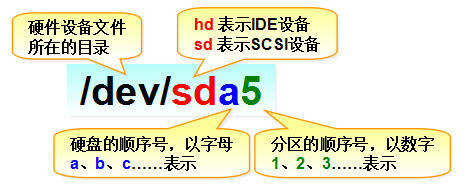
\includegraphics{Hard_disk_naming_convention.png}
		\caption{磁盘命名规则}
	\end{figure}
	
	首先,/dev/ 目录中保存的应当是硬件设备文件;其次,sd 表示的是存储设备;然后,a 表示系统中同类接口中第一个被识别到的设备;最后,5 表示这个设备是一个逻辑分区。因此,"/dev/sda5"表示的就是“这是系统中第一块被识别到的硬件设备中分区编号为5的逻辑分区的设备文件”。
	
	接下来我们科普一下硬盘相关的知识,包括主分区、扩展分区和逻辑分区的概念。
	
	\section{硬盘设备的内部存储结构}
	
	硬盘设备是由大量的扇区组成,每个扇区的容量为512字节。其中第一个扇区最重要,它里面保存着主引导记录与分区表信息。就第一个扇区来说,主引导记录需要占用446字节,分区表占用64字节,结束符占用2字节。其中分区表中每个记录一个分区信息就需要16字节,这样一来最多只有4个分区信息可以写到第一个扇区中,这4个分区就是4个主分区。
	
	\begin{figure}[htbp]
		\centering
		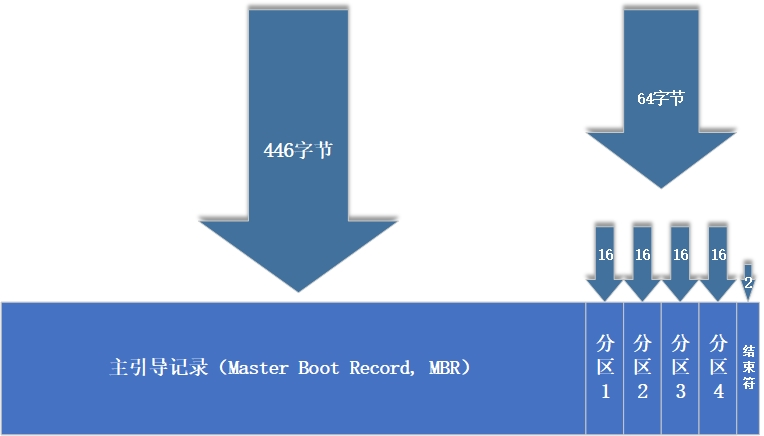
\includegraphics[scale=0.5]{first_sector.jpg}
		\caption{第一个扇区中的数据信息}
	\end{figure}
	
	但是,每块硬盘最多只能创建出4个分区,这明显不合情理也不够用!
	
	于是为了解决分区个数不够的问题,可以将第一个扇区的分区表中16个字节的空间拿出来指向另外一个分区(这个拿来指向另外一个分区的16字节的分区,我们称之为扩展分区)。也就是说,扩展分区其实并不是一个真正的分区,而更像是一个占用16字节分区表空间的指针(一个指向另一个分区的指针)。这样一来,用户一般会选择使用3个主分区加一个扩展分区的方式,然后在扩展分区中创建出数个逻辑分区,从而来满足多分区(大于4个)的需求。
	
	\emph{所谓扩展分区,严格地讲它不是一个实际意义的分区,而仅仅是一个指向其他分区的指针,这种指针结构将形成一个单向链表。因此扩展分区自身不能存储数据,用户需要在其指向的对应分区(称之为逻辑分区)上进行操作。}
	
	\begin{figure}[H]
		\centering
		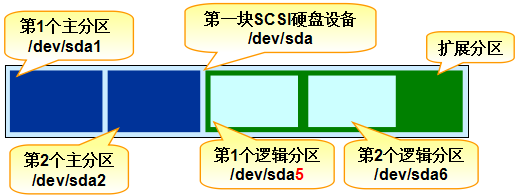
\includegraphics{Hard_disk_partitioning_rules.png}
		\caption{硬盘分区规则}
	\end{figure}
	
	
	\section{文件系统与数据资料}
	
	用户在硬件存储设备中执行的文件建立、写入、读取、修改、转存与控制等操作都是依靠文件系统来完成的。就像我们在A4纸上写字,如果随便写,就可能写的越来越歪,一行字不在同一横线上,那么为了让字写得更工整,阅读得更舒服一些,文具店里提供了各种不同的本本(单线本、双线本、田字格、五线谱等)。文件系统的作用是合理规划硬盘,以保证用户正常的使用需求。
	
	Linux系统支持数十种文件系统,而最常见的文件系统如下所示。
	
	\textbf{Ext2}:最早可追溯到1993年,是Linux系统的第一个商业级文件系统,它基本沿袭了UNIX文件系统的设计标准。但由于不包含日志读写功能,数据丢失的可能性很大,因此大家能不用就不用,或者顶多建议用于SD存储卡或U盘。
	
	\textbf{Ext3}:是一款日志文件系统,它会把整个硬盘的每个写入动作的细节都预先记录下来,然后再进行实际操作,以便在发生异常宕机后能回溯追踪到被中断的部分。Ext3能够在系统异常宕机时避免文件系统资料丢失,并能自动修复数据的不一致与错误。然而,当硬盘容量较大时,所需的修复时间也会很长,而且也不能100%地保证资料不会丢失。
	
	\textbf{Ext4}:Ext3的改进版本,作为RHEL 6系统中默认的文件管理系统,它支持的存储容量高达1EB(1EB=1,073,741,824GB),且能够有无限多的子目录。另外,Ext4文件系统能够批量分配block(块),从而极大地提高了读写效率。现在很多主流服务器也会使用Ext4文件系统。
	
	\textbf{XFS}:是一种高性能的日志文件系统,而且是RHEL 7/8中默认的文件管理系统。它的优势在发生意外宕机后尤其明显,即可以快速地恢复可能被破坏的文件,而且强大的日志功能只需花费极低的计算和存储性能。它支持的最大存储容量为18EB,这几乎满足了所有需求。
	
	
	\emph{在拿到一块新的硬盘存储设备后,先需要分区,然后再格式化文件系统,最后才能挂载并正常使用。硬盘分区操作取决于你的需求和硬盘大小;也可以选择不进行分区,但是必须对硬盘进行格式化处理。就像拿到了一张未裁切的完整纸张那样,首先要进行裁切以方便实用(分区),接下来在裁切后的纸张上画个以方便能书写工整(格式化),最后是正式使用(挂载)。}
	
	
	\section{挂载硬件设备}
	
	平时我们用惯Windows系统后觉得一切的操作都是理所当然的,平时把U盘插入到电脑后从来不会考虑Windows系统做了哪些事情,才使我们可以访问这个U盘。接下来我们看看在Linux系统中挂载和卸载存储设备的方法,以便大家更好地了解Linux系统添加硬件设备的工作原理和流程。
	
	前面讲到,在拿到一块新的硬盘存储设备后要先分区,然后格式化,最后才能挂载并正常使用。“分区”和“格式化”我们有所了解,那么“挂载”又是什么呢?
	
	\emph{当用户需要使用硬盘设备或者分区中的数据时,需要将其与一个已经存在的目录文件进行关联,而这个关联的动作就是“挂载”。}
	
	mount 命令用于挂载文件系统,格式为" \textbf{mount 文件系统 挂载目录}"。mount命令中可用的参数及作用如下表所示,挂载是在使用硬件设备前所执行的最后一步操作。只需使用mount命令把硬盘设备或分区与一个目录文件进行关联,然后就能在这个目录中看到硬件设备中的数据了。对于比较新的Linux系统来讲,一般不需要使用-t参数来指定文件系统的类型,Linux系统会自动进行判断。而mount中的-a参数则厉害了,它会在执行后自动检查/etc/fstab文件中有无被疏漏挂载的设备文件,如果有,则进行自动挂载操作。
	
	\begin{table}
		\centering
		\caption{mount命令参数}
		\begin{tabular}{ll}
			\hline
			参数 & 作用 \\
			\hline
			-a & 挂载所有在/etc/fstab中定义的文件系统\\
			-t & 指定文件系统的类型 \\
			\hline
		\end{tabular}
	\end{table}
	
	
	例如,要把设备/dev/sdb2挂载到/backup目录,只需要在mount命令中填写设备与挂载目录参数就行,系统会自动判断要挂载文件的类型,命令如下:
	
	\begin{lstlisting}
		$ mount /dev/sdb2 /backup
	\end{lstlisting}
	
	如果在工作中要挂载一块网络存储设备,该设备的名字可能会变来变去,这样再写为sdb就不太合适了。这时推荐用UUID(Universally Unique Identifier,通用唯一识别码)进行挂载操作。UUID是一串用于标识每块独立硬盘的字符串,具有唯一性及稳定性,特别适合用来挂载网络设备。使用blkid命令,能得知独立硬盘的UUID。
	
	\begin{lstlisting}
		$ blkid
		/dev/sdb1: UUID="2db66eb4-d9c1-4522-8fab-ac074cd3ea0b" TYPE="xfs" PARTUUID="eb23857a-01"
		/dev/sdb2: UUID="478fRb-1pOc-oPXv-fJOS-tTvH-KyBz-VaKwZG" TYPE="ext4" PARTUUID="eb23857a-02"
	\end{lstlisting}
	
	有了设备的UUID值之后,就可以用它挂载网络设备了:
	
	\begin{lstlisting}
		$ mount UUID=478fRb-1pOc-oPXv-fJOS-tTvH-KyBz-VaKwZG /backup
	\end{lstlisting}
	
	
	虽然按照上面的方法执行mount命令后就能立即使用文件系统了,但系统在重启后挂载就会失效,也就是说需要每次开机后都手动挂载一下。这肯定不是我们想要的效果,如果想让硬件设备和目录永久地进行自动关联,就必须把挂载信息按照指定的填写格式“设备文件 挂载目录 格式类型 权限选项 是否备份 是否自检”写入到/etc/fstab文件中。这个文件中包含着挂载所需的诸多信息项目,一旦配置好之后就能一劳永逸了。
	
	\begin{table}
		\centering
		\caption{fstab文件各字段的含义}
		\begin{tabular}{ll}
			\hline
			字段 & 意义 \\
			\hline
			设备文件 & 一般为设备的路径+设备名称,也可以写唯一识别码(UUID,Universally Unique Identifier) \\
			挂载目录 & 指定要挂载到的目录,需在挂载前创建好 \\
			格式类型 & 指定文件系统的格式,比如Ext3、Ext4、XFS、SWAP、iso9660(此为光盘设备)等 \\
			权限选项 & 若设置为defaults,则默认权限为:rw, suid, dev, exec, auto, nouser, async \\
			是否备份 & 若为1则开机后使用dump进行磁盘备份,为0则不备份 \\
			是否自检 & 若为1则开机后自动进行磁盘自检,为0则不自检 \\
			\hline
		\end{tabular}
	\end{table}
	
	如果想将文件系统为Ext4的硬件设备/dev/sdb2在开机后自动挂载到/backup目录上,并保持默认权限且无须开机自检,就需要在/etc/fstab文件中写入下面的信息,这样在系统重启后也会成功挂载。
	
	\begin{lstlisting}
		$ vim /etc/fstab
		#
		# /etc/fstab
		# Created by anaconda on Tue Jul 21 05:03:40 2020
		#
		# Accessible filesystems, by reference, are maintained under '/dev/disk/'.
		# See man pages fstab(5), findfs(8), mount(8) and/or blkid(8) for more info.
		#
		# After editing this file, run 'systemctl daemon-reload' to update systemd
		# units generated from this file.
		#
		/dev/mapper/rhel-root                     /        xfs     defaults    0 0
		UUID=812b1f7c-8b5b-43da-8c06-b9999e0fe48b /boot    xfs     defaults    0 0
		/dev/mapper/rhel-swap                     swap     swap    defaults    0 0
		/dev/sdb2                                 /backup  ext4    defaults    0 0
	\end{lstlisting}
	
	写入到/etc/fstab文件中的设备信息并不会立即生效,需要使用mount -a参数进行自动挂载:
	
	\begin{lstlisting}
		$ mount -a
	\end{lstlisting}
	
	df命令用于查看已挂载的磁盘空间使用情况,英文全称为"disk free",语法格式为"df -h" 。用 -h 参数便捷地对存储容量进行“进位”操作。例如,在遇到10240K的时候会自动进位写成10M,非常方便我们的阅读。
	
	\begin{lstlisting}
		$ df -h
		Filesystem      Size  Used Avail Use% Mounted on
		udev            3.6G     0  3.6G   0% /dev
		tmpfs           781M  1.9M  780M   1% /run
		/dev/mmcblk0p2   29G  3.3G   25G  12% /
		tmpfs           3.9G     0  3.9G   0% /dev/shm
		tmpfs           5.0M   16K  5.0M   1% /run/lock
		tmpfs           3.9G  4.0K  3.9G   1% /tmp
		/dev/mmcblk0p1  510M   96M  415M  19% /boot/firmware
		tmpfs           781M     0  781M   0% /run/user/1000	
	\end{lstlisting}
	
	
	
	说到网络存储设备,建议在fstab文件挂载信息中加上 \_netdev参数。加上后系统会等联网成功后再尝试挂载这块网络存储设备,从而避免了开机时间过长或失败的情况。
	
	\begin{lstlisting}
		$ vim /etc/fstab
		#
		# /etc/fstab
		# Created by anaconda on Tue Jul 21 05:03:40 2020
		#
		# Accessible filesystems, by reference, are maintained under '/dev/disk/'.
		# See man pages fstab(5), findfs(8), mount(8) and/or blkid(8) for more info.
		#
		# After editing this file, run 'systemctl daemon-reload' to update systemd
		# units generated from this file.
		#
		/dev/mapper/rhel-root                       /              xfs       defaults            0 0
		UUID=812b1f7c-8b5b-43da-8c06-b9999e0fe48b   /boot          xfs       defaults            0 0
		/dev/mapper/rhel-swap                       swap           swap      defaults            0 0
		/dev/sdb2                                   /backup        ext4      defaults,_netdev    0 0
		/dev/cdrom                                  /media/cdrom   iso9660   defaults            0 0
	\end{lstlisting}
	
	挂载文件系统的目的是为了使用硬件资源,而卸载文件系统则意味不再使用硬件的设备资源。既然挂载操作就是把硬件设备与目录两者进行关联的动作,那么卸载操作只需要说明想要取消关联的设备文件或挂载目录的其中一项即可,一般不需要加其他额外的参数。
	
	umount命令用于卸载设备或文件系统,英文全称为“un mount”,语法格式为“umount [设备文件/挂载目录]”。
	
	\begin{lstlisting}
		$ umount /dev/sdb2
	\end{lstlisting}
	
	\emph{如果我们当前就处于设备所挂载的目录,系统会提示该设备繁忙,此时只需要退出到其他目录后再尝试一次就行了。轻松搞定。}
	
	如果系统中硬盘特别多,分区特别多,我们都不知道它们是否有被使用,又或者是做了些什么。此时,就可以用lsblk命令以树状图的形式列举一下了。lsblk命令用于查看已挂载的磁盘的空间使用情况,英文全称为“list block id”,输入该命令后按回车键执行即可。
	
	\textbf{以下操作是在树莓派中执行的}
	
	\begin{lstlisting}
		pi@raspberrypi:~ $ lsblk
		NAME        MAJ:MIN RM   SIZE RO TYPE MOUNTPOINTS
		sda           8:0    0 465.8G  0 disk
		|-sda1        8:1    0     1K  0 part
		|-sda5        8:5    0 465.8G  0 part
		mmcblk0     179:0    0  29.7G  0 disk
		|-mmcblk0p1 179:1    0   512M  0 part /boot/firmware
		|-mmcblk0p2 179:2    0  29.2G  0 part /
	\end{lstlisting}
	
	
	\section{添加硬盘设备并使用}
	
	准备一块硬盘,插入到主机设备。这里就以我的树莓派为例,我通过树莓派USB3.0接口接入了一块机械硬盘。

	\begin{figure}[H]
		\centering
		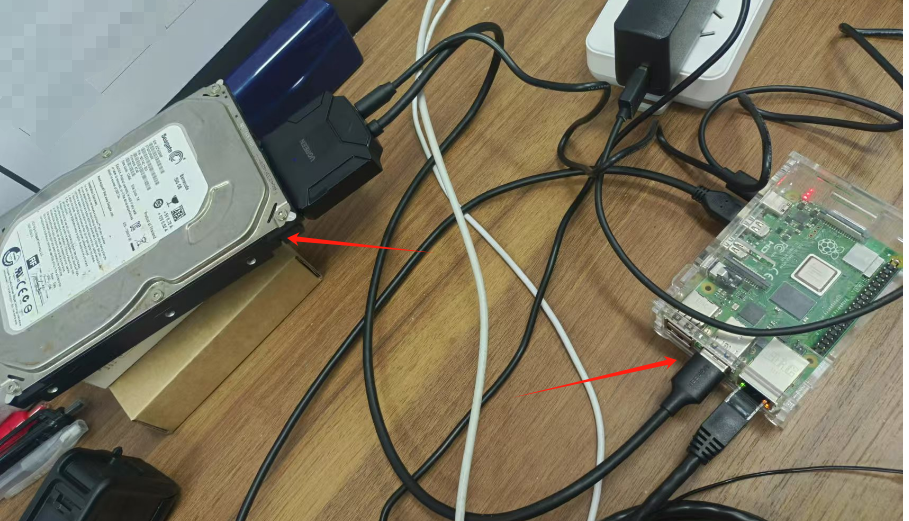
\includegraphics[scale=0.5]{my_drive.png}
		\caption{树莓派与外接的机械硬盘}
	\end{figure}
	
	通过lsblk命令可以看到这块硬盘的设备文件名是sda,并且里面有两个分区,编号分别是1和5(这是因为我接入的是一块二手硬盘,之前已经被分过区了)。
	
	那么接下来我想删除原有的分区,重新分区、格式化、挂载。
	
	fdisk命令用于新建、修改及删除磁盘的分区表信息,英文全称为“format disk”,语法格式为“fdisk 磁盘名称”。
	
	在Linux系统中,管理硬盘设备最常用的方法就当属fdisk命令了。它提供了集添加、删除、转换分区等功能于一身的“一站式分区服务”。不过与前面讲解的直接写到命令后面的参数不同,这条命令的参数是交互式的一问一答的形式,因此在管理硬盘设备时特别方便,可以根据需求动态调整。
	
	\begin{table}[H]
		\centering
		\caption{fdisk命令的参数}
		\begin{tabular}{ll}
			\hline
			参数 & 作用 \\
			\hline
			m & 查看全部可用的参数 \\
			n & 添加新的分区 \\
			d & 删除某个分区信息 \\
			l & 列出所有可用的分区类型 \\
			t & 改变某个分区的类型 \\
			p & 查看分区表信息 \\
			w & 保存并退出 \\
			q & 不保存直接退出 \\
			\hline
		\end{tabular}
	\end{table}
	
	首先使用fdisk命令来尝试管理/dev/sdb硬盘设备。在看到提示信息后输入参数p来查看硬盘设备内已有的分区信息,其中包括了硬盘的容量大小、扇区个数等信息:
	
	\begin{lstlisting}
		pi@raspberrypi:~ $ sudo fdisk /dev/sda
		
		Welcome to fdisk (util-linux 2.38.1).
		Changes will remain in memory only, until you decide to write them.
		Be careful before using the write command.
		
		
		Command (m for help): p
		Disk /dev/sda: 465.76 GiB, 500107862016 bytes, 976773168 sectors
		Disk model: 02-1BD142
		Units: sectors of 1 * 512 = 512 bytes
		Sector size (logical/physical): 512 bytes / 4096 bytes
		I/O size (minimum/optimal): 4096 bytes / 4096 bytes
		Disklabel type: dos
		Disk identifier: 0x797980c7
		
		Device     Boot Start       End   Sectors   Size Id Type
		/dev/sda1        2048 976773119 976771072 465.8G  f W95 Ext'd (LBA)
		/dev/sda5        4096 976773119 976769024 465.8G  7 HPFS/NTFS/exFAT
		
		Command (m for help):
	\end{lstlisting}
	
	
	在硬盘的分区信息中,我们可以看到 /dev/sda1 和 /dev/sda5 两个分区Size值是一样的,都是465.8G,但是上面我们通过lsblk命令查看磁盘的空间大小,发现/dev/sda1 的磁盘空间是1k ,而/dev/sda5 的磁盘空间是465.8G,这是怎么回事呢?
	
	从磁盘的信息我们可以看到,/dev/sda1的Type值是`W95 Ext'd (LBA)`,这说名/dev/sda1分区是扩展分区,而/dev/sda5是在这个扩展分区内划分的一个逻辑分区。扩展分区本身不直接用于存储数据,而是作为逻辑分区的容器。实际上,/dev/sda1作为扩展分区,其大小表示的是它所能容纳的逻辑分区空间的总和。而/dev/sda5作为这个扩展分区内的一个逻辑分区,被分配了与扩展分区剩余空间相等的逻辑容量。这两个分区在逻辑上大小相同,但实际上并不占用相同的物理空间。
	
	这里我先把原来的两个分区都删掉:
	
	\begin{lstlisting}
		Command (m for help): d
		Partition number (1,5, default 5):
		
		Partition 5 has been deleted.
		
		Command (m for help): d
		Selected partition 1
		Partition 1 has been deleted.
		
		Command (m for help): p
		Disk /dev/sda: 465.76 GiB, 500107862016 bytes, 976773168 sectors
		Disk model: 02-1BD142
		Units: sectors of 1 * 512 = 512 bytes
		Sector size (logical/physical): 512 bytes / 4096 bytes
		I/O size (minimum/optimal): 4096 bytes / 4096 bytes
		Disklabel type: dos
		Disk identifier: 0x797980c7
		
		Command (m for help):
		
	\end{lstlisting}
	
	然后创建一个主分区,并分配所有的磁盘空间:
	
	\begin{lstlisting}
		Command (m for help): n
		Partition type
		p   primary (0 primary, 0 extended, 4 free)
		e   extended (container for logical partitions)
		Select (default p): p
		Partition number (1-4, default 1):
		First sector (2048-976773167, default 2048):
		Last sector, +/-sectors or +/-size{K,M,G,T,P} (2048-976773167, default 976773167):
		
		Created a new partition 1 of type 'Linux' and of size 465.8 GiB.
		
		Command (m for help): p
		Disk /dev/sda: 465.76 GiB, 500107862016 bytes, 976773168 sectors
		Disk model: 02-1BD142
		Units: sectors of 1 * 512 = 512 bytes
		Sector size (logical/physical): 512 bytes / 4096 bytes
		I/O size (minimum/optimal): 4096 bytes / 4096 bytes
		Disklabel type: dos
		Disk identifier: 0x797980c7
		
		Device     Boot Start       End   Sectors   Size Id Type
		/dev/sda1        2048 976773167 976771120 465.8G 83 Linux
		
		Command (m for help):
		
	\end{lstlisting}
	
	设置分区类型:
	
	\begin{lstlisting}
		Command (m for help): t
		Selected partition 1
		Hex code or alias (type L to list all): 7
		Changed type of partition 'Linux' to 'HPFS/NTFS/exFAT'.
		
		Command (m for help): p
		Disk /dev/sda: 465.76 GiB, 500107862016 bytes, 976773168 sectors
		Disk model: 02-1BD142
		Units: sectors of 1 * 512 = 512 bytes
		Sector size (logical/physical): 512 bytes / 4096 bytes
		I/O size (minimum/optimal): 4096 bytes / 4096 bytes
		Disklabel type: dos
		Disk identifier: 0x797980c7
		
		Device     Boot Start       End   Sectors   Size Id Type
		/dev/sda1        2048 976773167 976771120 465.8G  7 HPFS/NTFS/exFAT
		
		Command (m for help):
		
	\end{lstlisting}
	
	最后保存设置的分区:
	
	\begin{lstlisting}
		Command (m for help): w
		The partition table has been altered.
		Calling ioctl() to re-read partition table.
		Syncing disks.
		
	\end{lstlisting}
	
	
	在上述步骤执行完毕之后,Linux系统会自动把这个硬盘主分区抽象成/dev/sdb1设备文件。可以使用file命令查看该文件的属性,但有些时候系统并没有自动把分区信息同步给Linux内核。可以输入partprobe命令手动将分区信息同步到内核,而且一般推荐连续两次执行该命令,效果会更好。如果使用这个命令都无法解决问题,那么就重启计算机吧。
	
	\begin{lstlisting}
		pi@raspberrypi:~ $ file /dev/sdb1
		/dev/sdb1: cannot open `/dev/sdb1' (No such file or directory)
		pi@raspberrypi:~ $ partprobe
		pi@raspberrypi:~ $ partprobe
		pi@raspberrypi:~ $ file /dev/sdb1
		/dev/sdb1: block special
	\end{lstlisting}
	
	如果硬件存储设备没有进行格式化,则Linux系统无法得知怎么在其上写入数据。因此,在对存储设备进行分区后还需要进行格式化操作。在Linux系统中用于格式化操作的命令是mkfs。这条命令很有意思,因为在Shell终端中输入mkfs名后再敲击两下用于补齐命令的Tab键,会有如下所示的效果:
	
	\begin{lstlisting}
		pi@raspberrypi:~ $ mkfs
		mkfs         mkfs.btrfs   mkfs.ext2    mkfs.ext4    mkfs.fat     mkfs.minix   mkfs.ntfs    mkfs.xfs
		mkfs.bfs     mkfs.cramfs  mkfs.ext3    mkfs.f2fs    mkfs.jfs     mkfs.msdos   mkfs.vfat
	\end{lstlisting}
	
	因为我们的分区设置的为`HPFS/NTFS/exFAT`类型,所以使用 mkfs.ntfs 进行格式化:
	
	\begin{lstlisting}
		pi@raspberrypi:~ $ sudo mkfs.ntfs /dev/sda1
		Cluster size has been automatically set to 4096 bytes.
		Initializing device with zeroes:  40%
		
	\end{lstlisting}
	
	\emph{注意:需要确保以root用户身份运行mkfs命令,因为普通用户没有权限格式化磁盘分区。}
	
	格式化完成
	
	\begin{lstlisting}
		pi@raspberrypi:~ $ sudo mkfs.ntfs /dev/sda1
		Cluster size has been automatically set to 4096 bytes.
		Initializing device with zeroes: 100% - Done.
		Creating NTFS volume structures.
		mkntfs completed successfully. Have a nice day.
		
	\end{lstlisting}
	
	终于完成了存储设备的分区和格式化操作,接下来就是要来挂载并使用存储设备了。与之相关的步骤也非常简单:首先是创建一个用于挂载设备的挂载点目录;然后使用mount命令将存储设备与挂载点进行关联;最后使用df -h命令来查看挂载状态和硬盘使用量信息。
	
	\begin{lstlisting}
		pi@raspberrypi:~ $ lsblk
		NAME        MAJ:MIN RM   SIZE RO TYPE MOUNTPOINTS
		sda           8:0    0 465.8G  0 disk
		|-sda1        8:1    0 465.8G  0 part
		mmcblk0     179:0    0  29.7G  0 disk
		|-mmcblk0p1 179:1    0   512M  0 part /boot/firmware
		|-mmcblk0p2 179:2    0  29.2G  0 part /
		pi@raspberrypi:~ $ mkdir /newFolder
		mkdir: cannot create directory '/newFolder': Permission denied
		pi@raspberrypi:~ $ sudo mkdir /newFolder
		pi@raspberrypi:~ $ mount /dev/sda1 /newFolder/
		mount: /newFolder: must be superuser to use mount.
		dmesg(1) may have more information after failed mount system call.
		pi@raspberrypi:~ $ sudo mount /dev/sda1 /newFolder/
		pi@raspberrypi:~ $ df -h
		Filesystem      Size  Used Avail Use% Mounted on
		udev            3.6G     0  3.6G   0% /dev
		tmpfs           781M  1.9M  780M   1% /run
		/dev/mmcblk0p2   29G  3.3G   25G  12% /
		tmpfs           3.9G     0  3.9G   0% /dev/shm
		tmpfs           5.0M   16K  5.0M   1% /run/lock
		tmpfs           3.9G  4.0K  3.9G   1% /tmp
		/dev/mmcblk0p1  510M   96M  415M  19% /boot/firmware
		tmpfs           781M     0  781M   0% /run/user/1000
		/dev/sda1       466G   79M  466G   1% /newFolder
	\end{lstlisting}
	
	du命令用查看分区或目录所占用的磁盘容量大小,英文全称为“disk usage”,语法格式为“du -sh目录名称”。
	
	既然存储设备已经顺利挂载,接下来就可以尝试通过挂载点目录向存储设备中写入文件了。在写入文件之前,先来看一个用于查看文件数据占用量的du命令。简单来说,该命令就是用来查看一个或多个文件占用了多大的硬盘空间。
	
	\emph{这里会发现,新硬盘刚挂载到指定目录,就有79M 的空间被使用,这是怎么回事?}
	
	\emph{这还是因为,当格式化硬盘兵创建爱你文件系统时,会有一部分空间用于存储文件系统的元数据,比如inode表、超级块等。这部分空间是用来维护文件系统结构的,对用户来说是不可见的。某些文件系统(如ext4)会保留一部分空间给超级用户(root)使用,以确保系统不会耗尽磁盘空间而导致无法写入重要的系统文件。如果你的硬盘上创建了交换空间或者系统恢复信息,那么这部分空间也会被标记为已使用。另外硬盘上的分区表也会占用一些空间,虽然通常很小。即使是一个空的目录,也会在文件系统中占用一些空间来存储目录信息,虽然占用的空间比较小。}
	
	前面在讲解mount命令时提到,使用mount命令挂载的设备文件会在系统下一次重启的时候失效。如果想让这个设备文件的挂载永久有效,则需要把挂载的信息写入配置文件中。
	
	这里我打算使用UUID进行挂载操作,那么首先使用 `blkid` 命令查询 /dev/sda1 的UUID。
	
	\begin{lstlisting}
		pi@raspberrypi:~ $ blkid
		/dev/mmcblk0p1: LABEL_FATBOOT="bootfs" LABEL="bootfs" UUID="4F7A-F93F" BLOCK_SIZE="512" TYPE="vfat" PARTUUID="543ffa18-01"
		/dev/mmcblk0p2: LABEL="rootfs" UUID="bb15c8e6-d999-4838-be67-5ff200bffa46" BLOCK_SIZE="4096" TYPE="ext4" PARTUUID="543ffa18-02"
	\end{lstlisting}
	
	这里又发现一个问题,/dev/sda1 这个设备没有显示出来。那么解决办法是,使用`sudo blkid`进行查询,发现可以查询到 /dev/sda1 设备的UUID信息,并且在这之后,再直接使用`blkid`命令,也会返回该设备的UUID。
	
	\begin{lstlisting}
		pi@raspberrypi:~ $ sudo blkid
		/dev/mmcblk0p1: LABEL_FATBOOT="bootfs" LABEL="bootfs" UUID="4F7A-F93F" BLOCK_SIZE="512" TYPE="vfat" PARTUUID="543ffa18-01"
		/dev/mmcblk0p2: LABEL="rootfs" UUID="bb15c8e6-d999-4838-be67-5ff200bffa46" BLOCK_SIZE="4096" TYPE="ext4" PARTUUID="543ffa18-02"
		/dev/sda1: BLOCK_SIZE="512" UUID="3AF716CB72002ECF" TYPE="ntfs" PARTUUID="797980c7-01"
		pi@raspberrypi:~ $ blkid
		/dev/mmcblk0p1: LABEL_FATBOOT="bootfs" LABEL="bootfs" UUID="4F7A-F93F" BLOCK_SIZE="512" TYPE="vfat" PARTUUID="543ffa18-01"
		/dev/mmcblk0p2: LABEL="rootfs" UUID="bb15c8e6-d999-4838-be67-5ff200bffa46" BLOCK_SIZE="4096" TYPE="ext4" PARTUUID="543ffa18-02"
		/dev/sda1: BLOCK_SIZE="512" UUID="3AF716CB72002ECF" TYPE="ntfs" PARTUUID="797980c7-01"
	\end{lstlisting}
	
	还有一种方法,是通过 lsblk -f 命令查询,也是可以看到UUID的。
	
	\begin{lstlisting}
		pi@raspberrypi:~ $ lsblk -f
		NAME        FSTYPE FSVER LABEL  UUID                                 FSAVAIL FSUSE% MOUNTPOINTS
		sda
		|-sda1      ntfs                3AF716CB72002ECF                      465.7G     0% /newFolder
		mmcblk0
		|-mmcblk0p1 vfat   FAT32 bootfs 4F7A-F93F                             414.8M    19% /boot/firmware
		|-mmcblk0p2 ext4   1.0   rootfs bb15c8e6-d999-4838-be67-5ff200bffa46   23.9G    12% /
		
	\end{lstlisting}
	
	最后,填写配置文件,使挂载永久生效。
	
	\begin{lstlisting}
		pi@raspberrypi:~ $ sudo vim /etc/fstab
		pi@raspberrypi:~ $ cat /etc/fstab
		proc            /proc           proc    defaults          0       0
		PARTUUID=543ffa18-01  /boot/firmware  vfat    defaults          0       2
		PARTUUID=543ffa18-02            /       ext4    noatime,nodiratime,defaults     0 1
		# a swapfile is not a swap partition, no line here
		#   use  dphys-swapfile swap[on|off]  for that
		
		UUID=3AF716CB72002ECF  /newFolder  ntfs  default  0  0
		
	\end{lstlisting}
	
	\section{交换分区}
	
	交换(SWAP)分区是一种通过在硬盘中预先划分一定的空间,然后把内存中暂时不常用的数据临时存放在硬盘中,以便腾出物理内存空间让更活跃的程序服务来使用的技术,其设计目的是为了解决真实物理内存不足的问题。通俗来讲就是让硬盘帮内存分担压力。但由于交换分区毕竟是通过硬盘设备读写数据的,速度肯定要比物理内存慢,所以只有当真实的物理内存耗尽后才会调用交换分区的资源。
	
	交换分区的创建过程与前文讲到的挂载并使用存储设备的过程非常相似。
	
	\emph{在生产环境中,交换分区的大小一般为真实物理内存的1.5~2倍。}
	
	\nocite{L:linuxprobe}
	
	\bibliographystyle{plain}
	\bibliography{references}
	
	
	
\end{document}